\section{熊野寮に入る人に一言言っておきたいこと}
\label{sec:kanadawasi}

\bunsekisha{文責}{銭苔}


私は、みなさんが熊野寮に入る前に覚えておいてほしいことがあります。とても簡単なことなので、気張らずに読んで下さい。

\centerline{\Large フライパンや鍋を金たわしでこすらないで}

スポンジでいくらこすっても焦げが取れないからって、すぐにフライパンや鍋を\ruby{金}{かな}だわし(スチールウール)でこすらないで。金だわしを使うと焦げが取れるだけでなく、フライパンや鍋表面の焦げ付き防止加工に傷が付きます。そうすると、フライパンや鍋は更に焦げ付きやすくなってしまいます。私はこれまでいくつもそうやって駄目になった共用の鍋やフライパンを見てきました。悲しいですね。

では焦げはどう取ればいいのでしょうか。まずは亀の子\ruby[g]{束子}{たわし}でこすってみましょう。これです。
\begin{figure}[H]
  \centering
  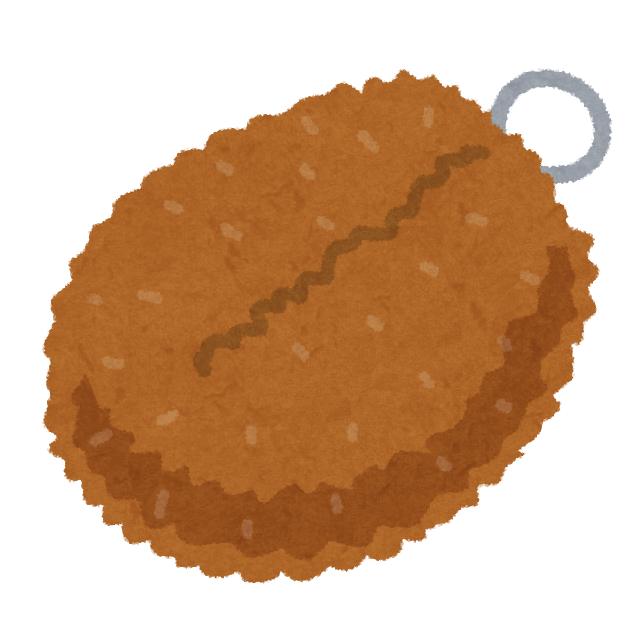
\includegraphics[width=4cm]{gazo/goods_tawashi.png}
\end{figure}
だいたいどこの\ruby{炊事場}{すい|じ|ば}にもあります。それでも取れなければ、1〜2時間程度水に浸けてからこすってみましょう。それでも取れなければ、マジックリンや重曹など共用の台所掃除用洗剤を説明書きを読みながら使ってみましょう。

いいですか。\emphbf{金だわしは最終手段です。}それを忘れないでください。

フライパンや鍋に限らず熊野寮には共用のものがたくさんあります。その多くが、寮生がなけなしのお金をはたいて寄付したものです。共用にした方がみんなにとって便利になるだろうという思いでそうするのです。しかし、買ったものがすぐに無残な姿になってしまえば、寄付した寮生の良心は裏切られ、もう二度と寄付をしてくれなくなるでしょう。こうしたことが度重なると自分のものは自分で所有したほうが良いという考えが蔓延し共用のものが減り、結果として新参者や貧乏人が暮らしにくい寮になってしまいます。

「共用のものは丁寧に繊細に扱え」とまでは言いません。共用のものに溢れている空間でその全てに気を配るのも、それはそれで大変です。私が言いたいのは、使い方を守りましょうということです。ネット検索なり人に訊ねるなりして、道具の使い方を習得してから使いましょうということです。あるいは、壊したら素直に申告して謝りましょうということです。あるいは、あなたも寄付をしましょうということです。

自戒を込めて